% The code is quite messy !!!

\documentclass[tikz,border=10pt]{standalone}

\begin{document}

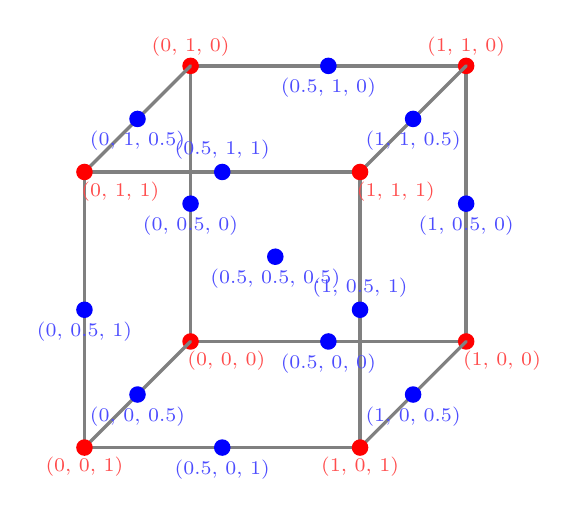
\begin{tikzpicture}[scale=3.5, line join=round, line cap=round]

    % Cube edges
    \draw[gray, very thick] (0,0,0) -- (1,0,0) -- (1,1,0) -- (0,1,0) -- cycle;
    % Vertices (corners)
    \foreach \x/\y/\z in {0/0/0, 1/0/0, 1/1/0, 0/1/0} {
        \fill[red] (\x,\y,\z) circle (0.03);
    }
    \draw[gray, very thick] (0,0,0) -- (0,0,1);
    \draw[gray, very thick] (1,0,0) -- (1,0,1);
    \draw[gray, very thick] (1,1,0) -- (1,1,1);
    \draw[gray, very thick] (0,1,0) -- (0,1,1);
    \draw[gray, very thick] (0,0,1) -- (1,0,1) -- (1,1,1) -- (0,1,1) -- cycle;

   % Vertices (corners)
   \foreach \x/\y/\z in {0/0/1, 1/0/1, 1/1/1, 0/1/1} {
        \fill[red] (\x,\y,\z) circle (0.03);
    }

    % Vertices (Face centers)
    \foreach \x/\y/\z in {0.5/0.5/0.5, 0.5/0/0, 0.5/1/0, 0.5/0/1, 0.5/1/1, 0/0.5/0, 1/0.5/0, 0/0.5/1, 1/0.5/1, 0/0/0.5, 1/0/0.5, 0/1/0.5, 1/1/0.5} {
        \fill[blue] (\x,\y,\z) circle (0.03);
    }

    % coordinates (corners)
   \foreach \x/\y/\z in {0/0/1, 1/0/1} {
        \node[red!70!white, font=\scriptsize] at (\x,\y-0.07,\z) {(\x, \y, \z)};
    }
    % coordinates (corners)
   \foreach \x/\y/\z in {0/0/0, 1/0/0, 1/1/1, 0/1/1} {
        \node[red!70!white, font=\scriptsize] at (\x+0.13,\y-0.07,\z) {(\x, \y, \z)};
    }
     % coordinates (corners)
    \foreach \x/\y/\z in {1/1/0, 0/1/0} {
        \node[red!70!white, font=\scriptsize] at (\x,\y+0.07,\z) {(\x, \y, \z)};
    }

    % coordinates (Face centers)
    \foreach \x/\y/\z in {0.5/0.5/0.5, 0.5/0/0, 0.5/1/0, 0.5/0/1, 0/0.5/0, 1/0.5/0, 0/0.5/1, 0/0/0.5, 1/0/0.5, 0/1/0.5, 1/1/0.5} {
        \node[blue!70!white, font=\scriptsize] at (\x,\y-0.08,\z) {(\x, \y, \z)};
    }
     % coordinates (Face centers)
     \foreach \x/\y/\z in {0.5/1/1, 1/0.5/1} {
        \node[blue!70!white, font=\scriptsize] at (\x,\y+0.08,\z) {(\x, \y, \z)};
    }
\end{tikzpicture}

\end{document}